%%%%%%%%%%%%%%%%%%%%%%%%%%%%%%%%%%%%%%%%%%%%%%%%%%%%%%%%%%%%%%%%%%%%%%%%%%%%%%%%
%%  Constitutive Model
%%%%%%%%%%%%%%%%%%%%%%%%%%%%%%%%%%%%%%%%%%%%%%%%%%%%%%%%%%%%%%%%%%%%%%%%%%%%%%%%


\section{Constitutive model for uncycled exogenously crosslinked tissue}

%%%%%%%%%%%%%%%%%%%%%%%%%%%%%%%%%%%%%%%%%%%%%%%%%%%%%%%%%%%%%%%%%%%%%%%%%%%%%%%%
%%%%    Constitutive Model for crosslinking

\subsection{Constitutive model for exogenous crosslinking}

	We have previously developed the first constitutive model for exogenously crosslinked collagenous tissues \cite{sacks_novel_2016} and determined the following three contributors to the mechanical response: collagen fibers, EXL matrix and fiber-fiber interactions, where the total strain energy density function is given by
\begin{equation} \label{eq:totalstrainenergy}
    \Psi = \phi_\mathrm{col} \left[ \Psi_\mathrm{col} + \Psi_\mathrm{int}\right] + \phi_m \Psi_m
\end{equation}
	In particular, we found the fiber ensemble interaction term ($\phi_\mathrm{col} \Psi_\mathrm{int}$) to be especially important in modeling exogenously crosslinked tissues, accounting for approximately 30\% of the stress in the fully loaded state (Fig. \ref{fig:EXLforms}A). To determine the model form of the interaction component, we used the remaining stress after subtracting the collagen fiber response and EXL matrix response from the mechanical response of the tissue after exogenous crosslinking (Fig. \ref{fig:EXLforms}A). In that study, we consider three possible forms of interactions: intra-fiber ensemble (Fig. \ref{fig:EXLforms}B) (an ensemble being a family of fibers sharing a common orientation), ensemble-ensemble rotations, and ensemble-ensemble relative extensions (Fig. \ref{fig:EXLforms}C\&D). We found that intra-fiber ensemble and ensemble-ensemble rotations were not consistent with the experimental data, whereas ensemble-ensemble extensional interactions were able to explain all of the remaining stress. 
	
\begin{figure}[hbt]
\centering
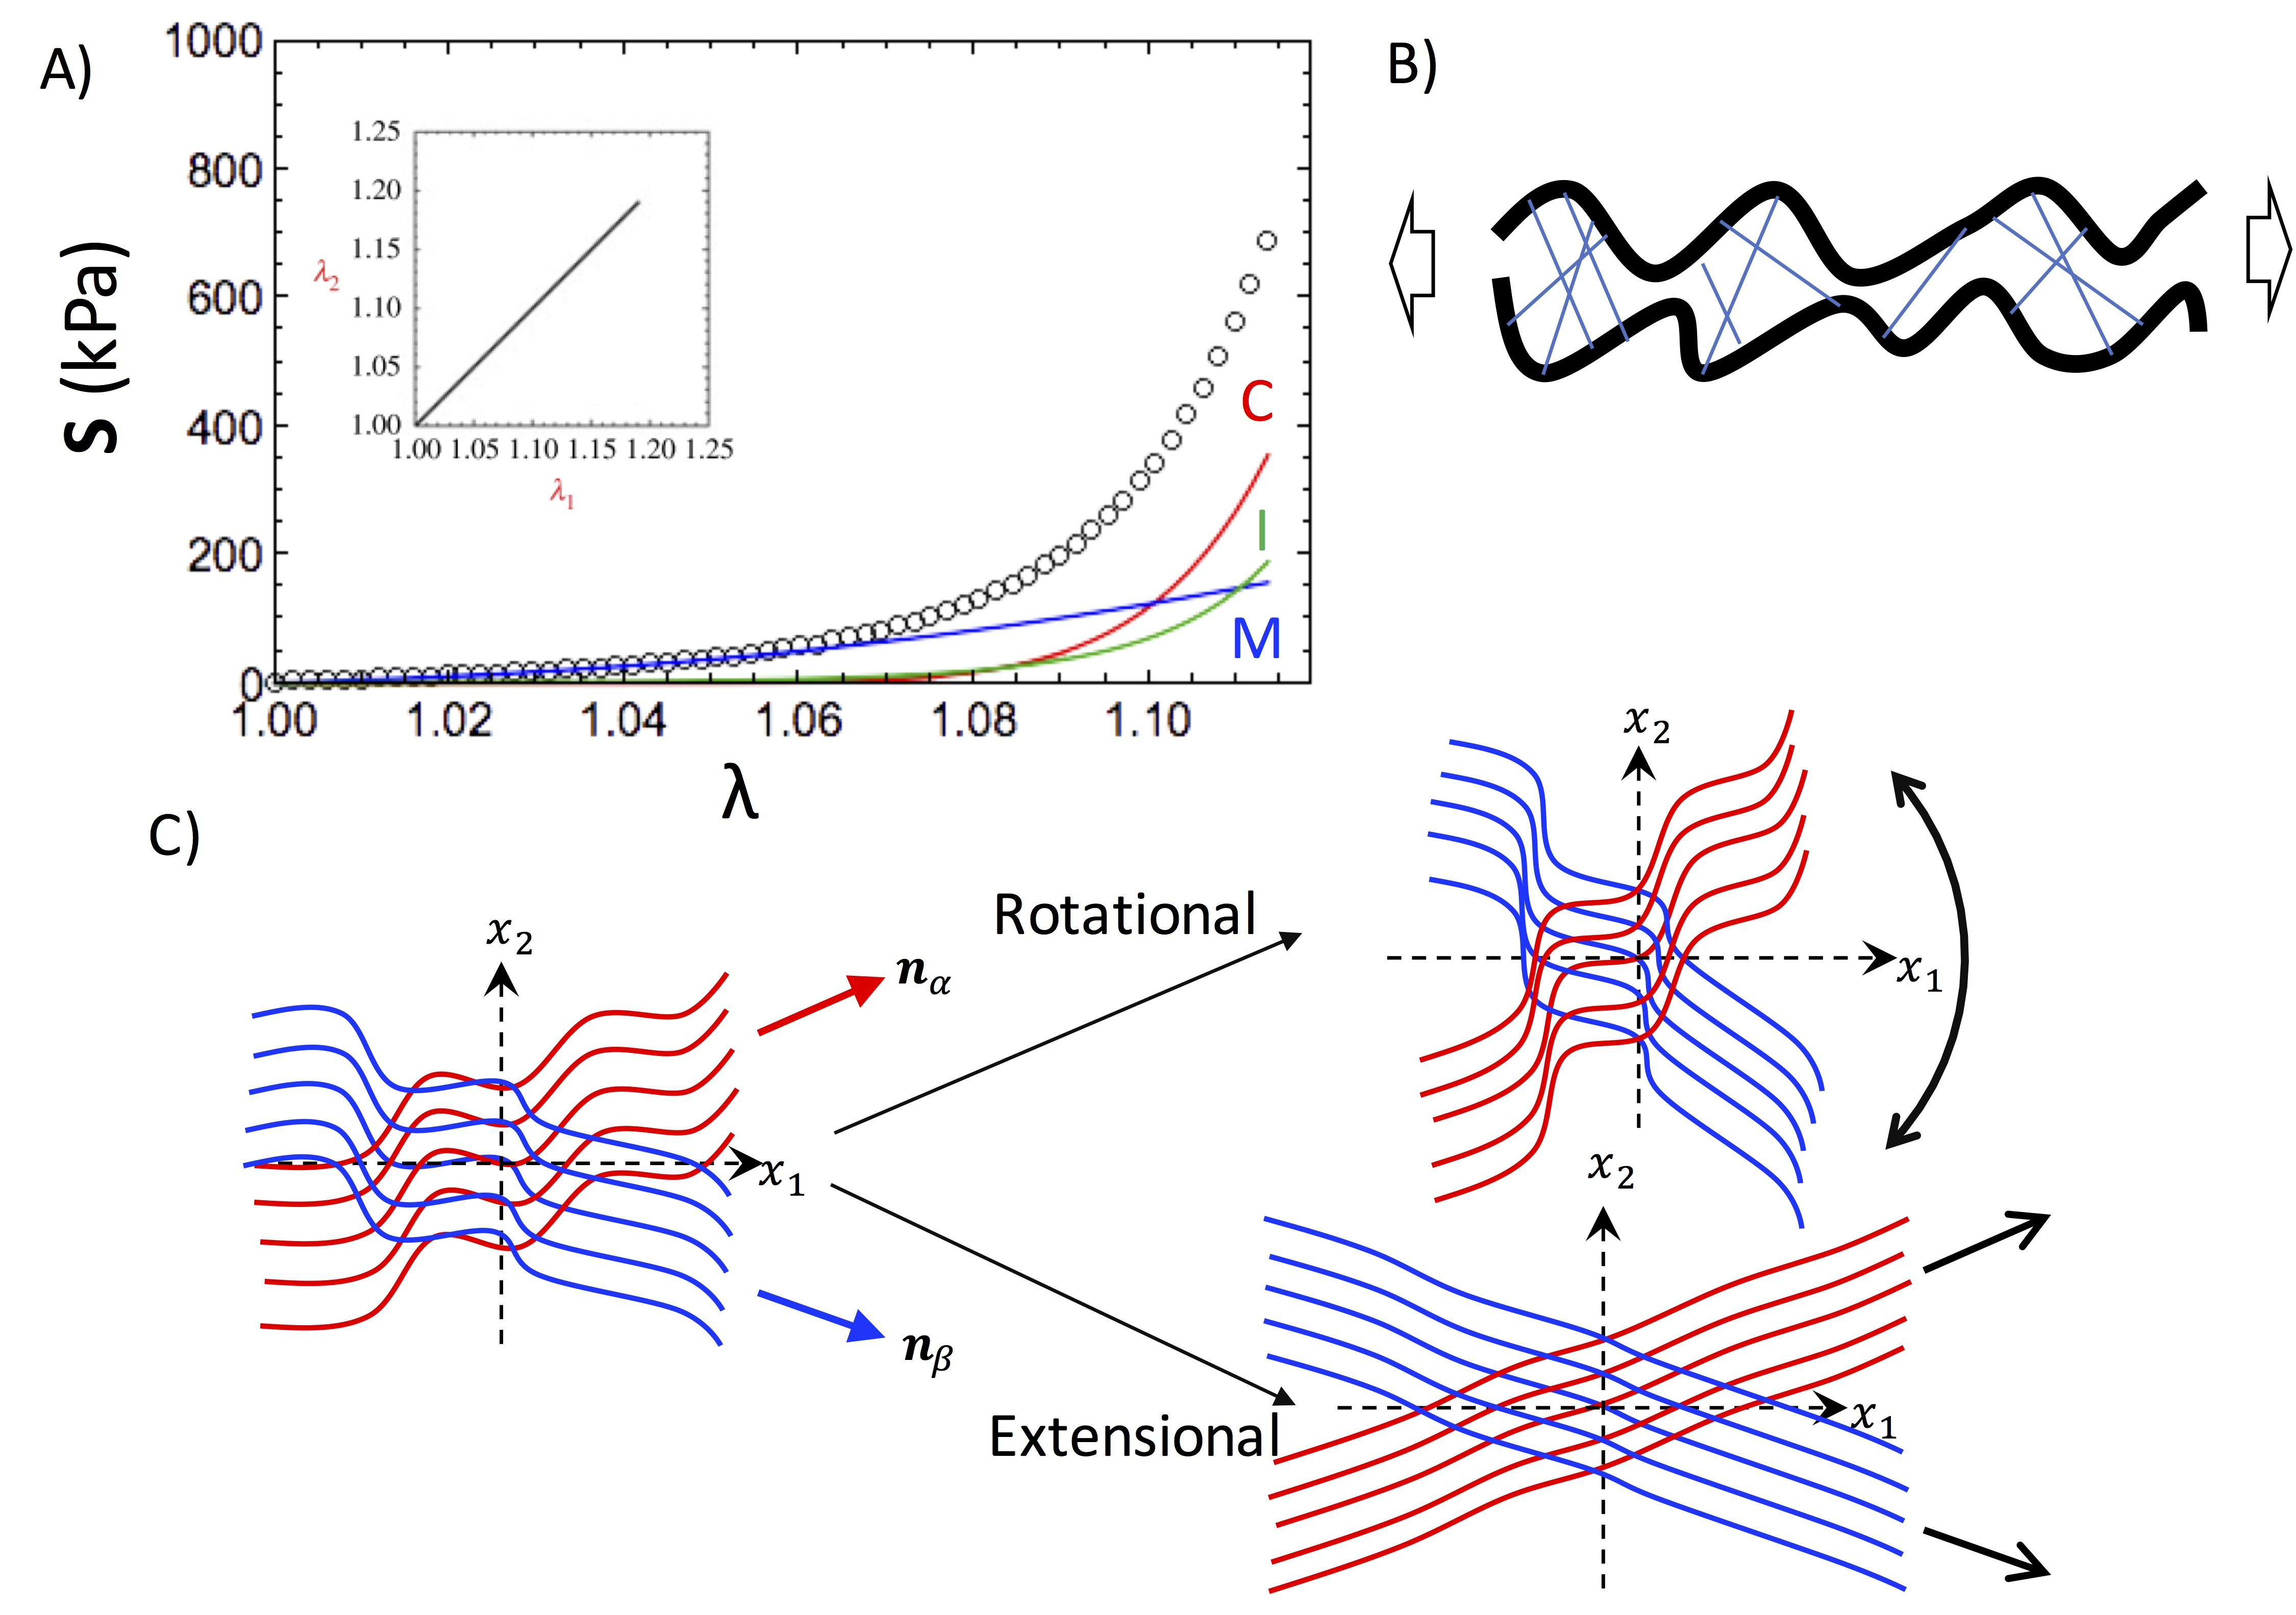
\includegraphics[width=\textwidth]{Images/chapter4/figure6}
\caption{A) The mechanical response of exogenously crosslinked BP, which is composed of 3 parts: (C)ollagen in Red, (M)atrix in Blue, and the fiber ensemble (I)nteractions in Green. B) Illustration for intra-ensemble interactions due to crosslinking is shown. C) The inter-ensemble interactions could be separated into rotational effects and extensional effects. }
\label{fig:EXLforms}
\end{figure}
	
    The interaction model form, $\Psi_\mathrm{int}$, was developed utilizing the pseudo invariant $I_8$, which is a function of the stretch and angle between two fiber ensembles oriented along the angle $\alpha$ and $\beta$ directions in the tissue (Fig. \ref{fig:structuralconvection}), and then separated it into its rotational and extensional components\cite{sacks_novel_2016} (Fig. \ref{fig:EXLforms}C\&D),
\begin{equation} \label{eq:I8invariant}
\begin{gathered}
I_8 = \mathbf{n}_ \alpha \cdot\mathbf{C}\cdot\mathbf{n}_\beta = \lambda_\alpha \lambda_\beta \cos(\alpha - \beta), \\
I_8^{\mathrm{ext}} = \lambda_\alpha \lambda_\beta, \qquad I_8^{\mathrm{rot}} = \cos(\alpha - \beta) = \frac{I_8}{\lambda_\alpha \lambda_\beta},
\end{gathered}
\end{equation}
    where $\mathbf{n}_\alpha$ and $\mathbf{n}_\beta$ are vectors pointing along $\alpha$ and $\beta$, respectively, $\lambda_\alpha$ and $\lambda_\beta$ are the stretches of the collagen fiber ensembles oriented along $\alpha$ and $\beta$, respectively , $I_8^\mathrm{ext}$ is the pseudo invariant for ensemble-ensemble extensions, and $I_8^\mathrm{rot}$ is the pseudo invariant for ensemble-ensemble rotations. From this, we established the model form for the interactions to be
\begin{equation}
\Psi_{\mathrm{int}} = \frac{d_0}{4}\int\displaylimits_\alpha \int\displaylimits_\beta \Gamma\left(\alpha\right)\Gamma \left( \beta \right)\left[ e^{d_1(\lambda_\alpha \lambda_\beta - 1)^2}-1 \right] \mathrm{d}\alpha\, \mathrm{d}\beta,
\end{equation}
    where $\Gamma$ is the fiber orientation distribution (ODF), and $d_0$ and $d_1$ are material constants. 
	However, this model form is still essentially phenomenological. 
	Specifically, while it is sufficient to model the mechanical response in the range of the acquired experimental data, we have no method for predicting how it will change with changes in dimensions with cyclic loading. Thus, an extension to this model component is necessary.

%%%%%%%%%%%%%%%%%%%%%%%%%%%%%%%%%%%%%%%%%%%%%%%%%%%%%%%%%%%%%%%%%%%%%%%%%%%%%%%%
%%%%    Extension for structural model

\subsection{Extension of the structural derivation of the fiber-fiber interactions term}

    The key to our approach in the constitutive model for the permanent set effect is to use the change in the collagen fiber architecture to predict the new mechanical response. Thus, having a full structural model, including a full structural derivation of the fiber-fiber interactions, is crucial. As in the previous model form \cite{sacks_novel_2016}, we will only keep the extensional component $I_8^\mathrm{ext}$. In addition, since collagen fibers do not bear stress until fully straightened \cite{soares_biomechanical_2016}, we also assume that \emph{collagen fibers do not play a role in the interactions of the fiber ensembles until they are straightened}. Following the same approach common in structural models, we first define the stretch of the collagen fibers after it's straightened, which is also the true fiber stretch ($\lambda_t$) defined in Zhang et al. \cite{zhang_meso_2016}, to be $\lambda_t = \lambda_\mathrm{ens}/\lambda_s$, where $\lambda_\mathrm{ens}$ is the stretch of the collagen fiber ensemble and $\lambda_s$ is the slack stretch required to straighten the collagen fiber crimp. We assumed that interactions do not occur until the fibers are straighten, so the extensional invariant should be a function of the true stretch of the individual fibers, $\lambda_t$, rather than the stretch of the whole fiber ensembles as defined in equation \ref{eq:I8invariant},
\begin{equation}
I_8^{\mathrm{ext}} = \frac{\lambda_\alpha \lambda_\beta}{\prescript{}{\alpha}{\lambda}_s \prescript{}{\alpha}{\lambda}_s},
\end{equation}
    where $\prescript{}{\alpha}{\lambda}_s$ and $\prescript{}{\beta}{\lambda}_s$ are the slack stretches of the two ensembles oriented along $\alpha$ and $\beta$ in the reference configuration, respectively. This invariant is then integrated only for fibers with $\lambda_t > 1$, i.e. fibers which are straightened. To develop the form for the interactions, we start from the strain energy. At the ensemble level, we integrate the invariant over the slack stretch $(\lambda_s)$ of both the fiber ensembles orienting along $\alpha$ and $\beta$, weighted by the probability distribution function of the proportion of collagen fibers with that specific slack stretch $D(\lambda_s)$,
\begin{equation}
\Psi_{\mathrm{int}}^{\mathrm{ens}} = \frac{\eta_I}{2} \int\displaylimits_1^{\lambda_\alpha} \int\displaylimits_1^{\lambda_\beta} D\left( x_\alpha \right) D\left( x_\beta \right) \left( \frac{\lambda_\alpha \lambda_\beta}{x_\alpha x_\beta} - 1\right)^2 \,\mathrm{d}x_\alpha \,\mathrm{d}x_\beta.
\end{equation}
    We refer to $D(\lambda_s)$ as the recruitment function, which is defined in Zhang et al. \cite{zhang_meso_2016}. The ensemble-level model is then integrated with respect to the fiber ODF, $\Gamma$, for all possible pair of collagen fiber ensemble to give the tissue-level model
\begin{equation}
\Psi_{\mathrm{int}} = \frac{\eta_I}{2} \int\displaylimits_\alpha \int\displaylimits_\beta \Gamma(\alpha) \Gamma(\beta) \int\displaylimits_1^{\lambda_\alpha} \int\displaylimits_1^{\lambda_\beta} D\left( x_\alpha \right) D\left( x_\beta \right) \left( \frac{\lambda_\alpha \lambda_\beta}{x_\alpha x_\beta} - 1\right)^2 \,\mathrm{d}x_\alpha \,\mathrm{d}x_\beta \,\mathrm{d}\alpha \,\mathrm{d}\beta.
\end{equation}
    The second Piola Kirchhoff stress, using $\mathbf{S}=2\frac{\partial\Psi}{\partial\mathbf{C}}$, is 
\begin{equation} \label{eq:interaction}
\begin{split}
\mathbf{S}_{\mathrm{int}} = \eta_I \int\displaylimits_\alpha \int\displaylimits_\beta \Gamma \left(\alpha \right) \Gamma \left( \beta \right) 
\left[ \left\lbrace 
\int\displaylimits_1^{\lambda_\alpha} \int\displaylimits_1^{\lambda_\beta} 
\frac{2 \lambda_\beta D(x_\alpha) D(x_\beta)}{x_\alpha x_\beta} 
\left( \frac{\lambda_\alpha}{x_\alpha} \frac{\lambda_\beta}{x_\beta} - 1\right) \mathrm{d}x_\alpha \, \mathrm{d}x_\beta \right.\right. +&\\
\left. \left. \int\displaylimits_1^{\lambda_\beta} D(x_\beta) \left( \frac{\lambda_\beta}{x_\beta} -1  \right)^2 \mathrm{d}x_\beta \right\rbrace \right.  \frac{\mathbf{n}_\alpha \otimes \mathbf{n}_\alpha}{\lambda_\alpha} +& \\
\left. \left\lbrace
\int\displaylimits_1^{\lambda_\alpha} \int\displaylimits_1^{\lambda_\alpha} 
\frac{2 \lambda_\beta D(x_\alpha) D(x_\beta)}{x_\alpha x_\beta} 
\left( \frac{\lambda_\alpha}{x_\alpha} \frac{\lambda_\beta}{x_\beta} - 1\right) \mathrm{d}x_\alpha \, \mathrm{d}x_\beta 
\right. \right. +&\\
\left. \left. \int\displaylimits_1^{\lambda_\alpha} D(x_\alpha) \left( \frac{\lambda_\alpha}{x_\alpha} -1  \right)^2 \mathrm{d}x_\alpha \right\rbrace \frac{\mathbf{n}_\beta \otimes \mathbf{n}_\beta}{\lambda_\beta}  \right]& \mathrm{d}\alpha \, \mathrm{d}\beta.
\end{split}
\end{equation}
    This model form has only one constant $\eta_I$ to account for all interactions. The remaining mechanisms are all based on the collagen fiber architecture, which is determined through a convection using dimensional changes. 